%!TEX root = ../../main.tex


\begin{figure}[!htb]
\centering
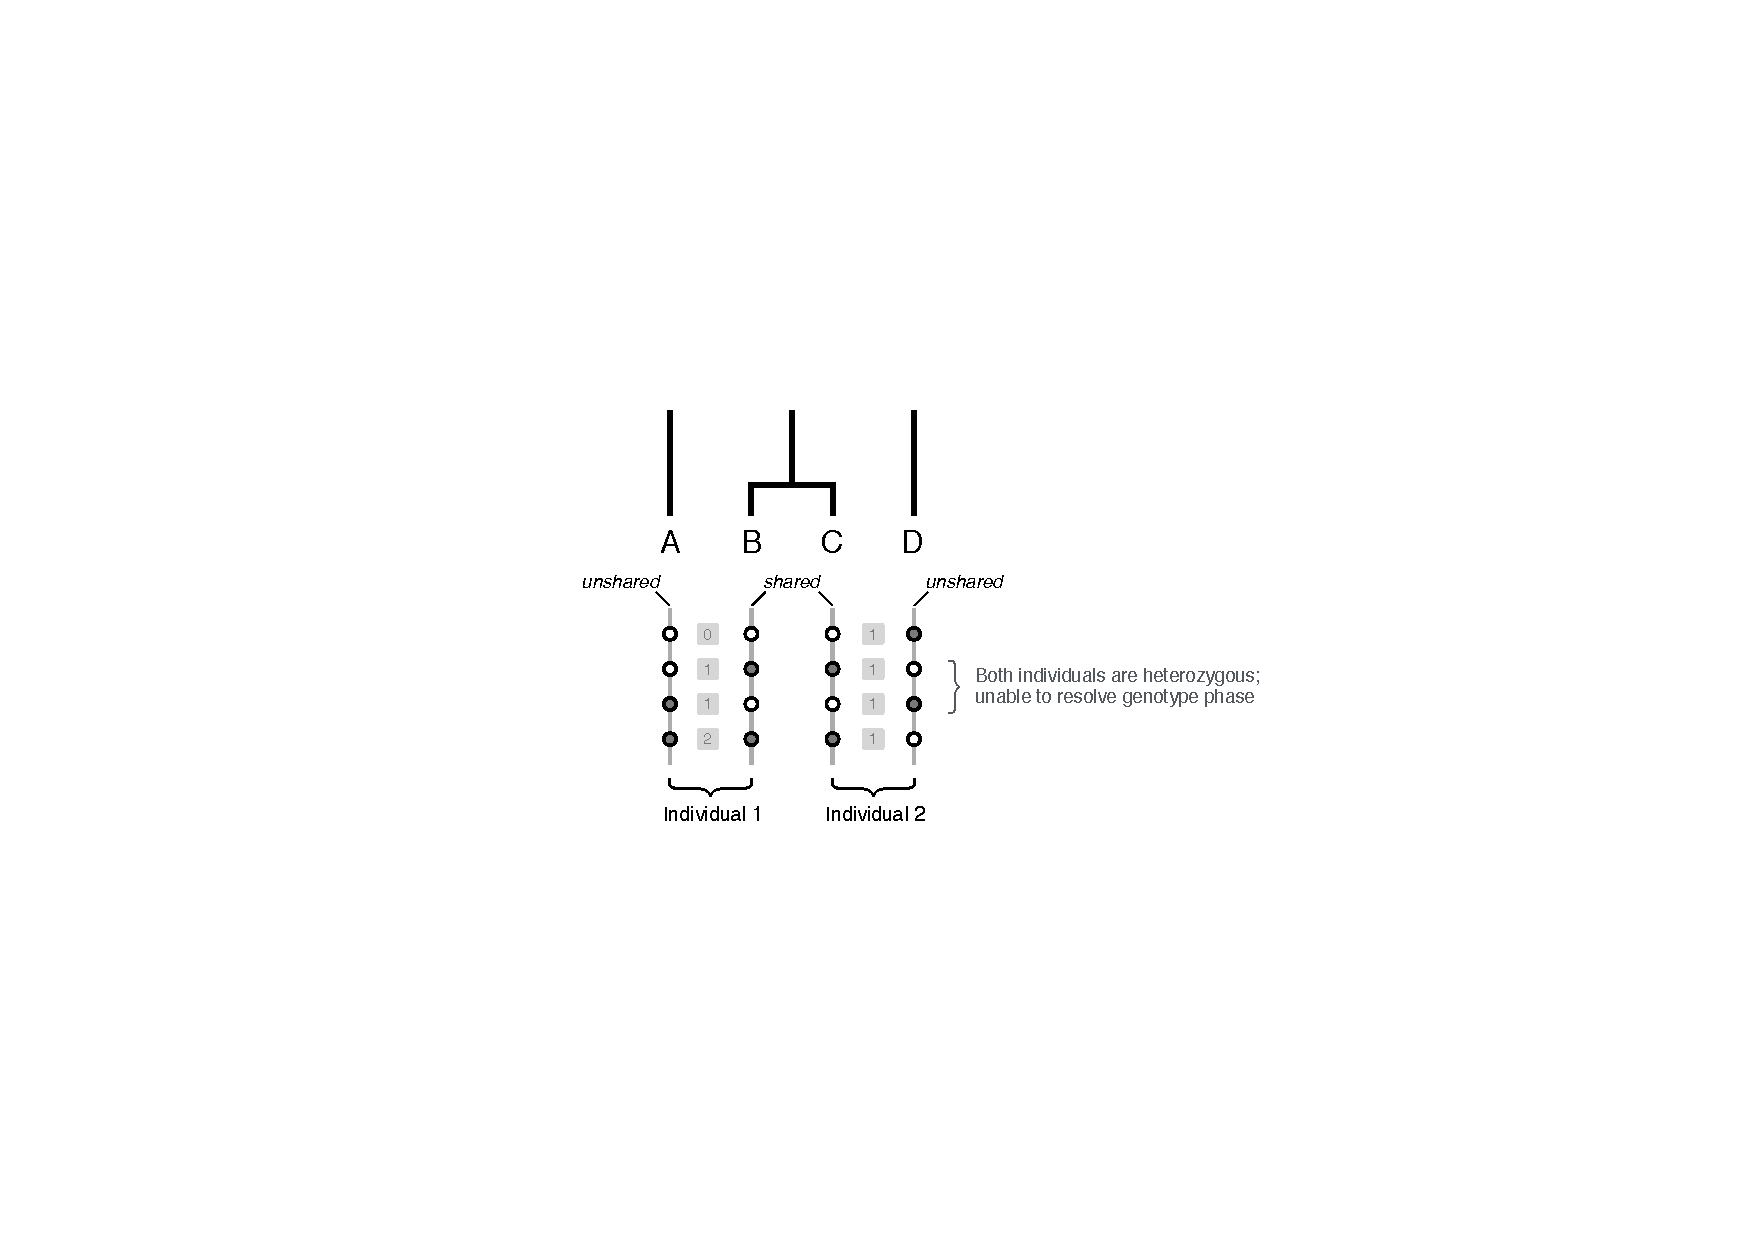
\includegraphics[width=0.75\textwidth]{./img/ch3/info_phase_pedigree}
\Caption{Genealogical constraints from haplotype sharing}
{The top graph indicates the genealogy of \n{4} haplotypes (A, B, C, and D) as seen in \n{2} individuals (1 and 2), which can be resolved partially if \n{2} haplotypes are shared by descent.
Below, the allelic states are shown at \n{4} positions along the sequence for each haplotype; ancestral and derived states are indicated by \emph{hollow} and \emph{solid} circles.
Only the genotypic state is seen in each individual as indicated between individual haplotypes; \ie homozygous for the ancestral allele (0), heterozygous (1), and homozygous for the derived allele (2).
The phase of a genotype can be resolved at sites with \n{1} homozygous genotype (phasing is redundant if both genotypes are homozygous).
Genotype phase cannot be determined if both individuals are heterozygous.}
{fig:info_phase_pedigree}
\end{figure}
